\chapter {IMPLEMENTASI}

\section{Lingkungan Implementasi}

Lingkungan implementasi dan pengembangan menggunakan sebuah komputer dengan spesifikasi perangkat lunak dan perangkat keras sebagai berikut.

\begin{enumerate}
	\item Perangkat Keras
	\par Implementasi tugas akhir ini menggunakan desktop personal computer ASUS X555Q. Namun digunakan untuk menjalankan Google Colab dengan spesifikasi :
	\begin{enumerate}
		\item GPU: 1x Tesla K80 , having 2496 CUDA cores, compute 3.7, 12GB(11.439GB Usable) GDDR5 VRAM
		\item CPU: 1x single core hyper threaded i.e(1 core, 2 threads) Xeon Processors @2.3Ghz (No Turbo Boost) , 45 MB Cache
	\end{enumerate}
	\item Perangkat Lunak
	\begin{enumerate}
		\item Sistem Operasi Linux 18.04 64-bit
		\item Android Studio
		\item Bahasa Pemrograman Java
		\item Bahasa Pemrograman Python
		\item Library Keras
	\end{enumerate}
\end{enumerate}

\section{Implementasi Ekstraksi Fitur}
Subbab ini menjabarkan implementasi ekstraksi fitur. 

\par Yang pertama dilakukan adalah mengatur konfigurasi. Konfigurasi yang dapat diatur antara lain nama model, bobot, train path atau direktori folder yang akan dilatih, features path atau direktori file untuk menyimpan fitur, label path atau direktori file untuk menyimpan label, test size atau perbandingan rasio antara data test dan data train, results atau direktori file untuk menyimpan hasil train keseluruhan. 
\begin{lstlisting}[language=java, caption=Konfigurasi, label=code:config, firstnumber=1]
{
"model"           : "mobilenet",
"weights"         : "imagenet",
"include_top"     : false,

"train_path"      : "../RGB",
"test_path"		  : "test",
"features_path"   : "mobilenet/features.h5",
"labels_path"     : "mobilenet/labels.h5",
"results"         : "mobilenet/results.txt",
"classifier_path" : "mobilenet/classifier.pickle",
"model_path"	  : "mobilenet/model",

"test_size"       : 0.3,
"seed"            : 9,
"num_classes"     : 42
}
\end{lstlisting}
\par Fungsi untuk membaca konfigurasi dari file berbentuk json. 
\mbox{}
\mbox{}
\begin{lstlisting}[language=python, caption=Membaca konfigurasi, label=code:open_config, firstnumber=37]
	with open('conf/conf.vgg19.json') as f:
	config = json.load(f)
	
	model_name = config["model"]
	weights = config["weights"]
	include_top = config["include_top"]
	train_path = config["train_path"]
	features_path = config["features_path"]
	labels_path = config["labels_path"]
	test_size = config["test_size"]
	results = config["results"]
	model_path = config["model_path"]
\end{lstlisting}


\begin{lstlisting}[language=python, caption=Menentukan arsitektur untuk ekstraksi fitur, label=code:choose_architecture, firstnumber=58]
if model_name == "vgg16":
base_model = VGG16(weights=weights)
model = Model(inputs=base_model.input, outputs=base_model.get_layer('fc1').output)
elif model_name == "vgg19":
base_model = VGG19(weights=weights)
model = Model(input=base_model.input, output=base_model.get_layer('fc1').output)

elif model_name == "resnet50":
base_model = ResNet50(weights=weights)
lastLayer = base_model.layers[-2]
model = Model(input=base_model.input, output=lastLayer.output) 

elif model_name == "inceptionv3":
base_model = InceptionV3(include_top=include_top, weights=weights, input_tensor=Input(shape=(299, 299, 3)))
output = base_model.output
model = Model(inputs=base_model.input, outputs=output)

elif model_name == "mobilenet":
base_model = MobileNet(include_top=include_top, weights=weights, input_tensor=Input(shape=(224, 224, 3)),
input_shape=(224, 224, 3))
output = base_model.output
model = Model(inputs=base_model.input, outputs=output)
elif model_name == "xception":
base_model = Xception(weights=weights)
model = Model(input=base_model.input, output=base_model.get_layer('avg_pool').output)
image_size = (299, 299)
else:
base_model = None
\end{lstlisting}
\par Fungsi untuk menentukan arsitektur apa yang akan digunakan untuk mengekstraksi fitur dari file konfigurasi json.

\begin{lstlisting}[language=python, caption=Preproses Data, label=code:preprocess, firstnumber=123]
count = 1
for i, label in enumerate(train_labels):
cur_path = train_path + "/" + label
count = 1
for image_path in glob.glob(cur_path + "/*.JPG"):
img = image.load_img(image_path, target_size=image_size)
x = image.img_to_array(img)
x = np.expand_dims(x, axis=0)
x = preprocess_input(x)
feature = model.predict(x)
flat = feature.flatten()  ### double flatten dg diatas
features.append(flat)
labels.append(label)
print("[INFO] processed - " + str(count))
count += 1
print("[INFO] completed label - " + label)
\end{lstlisting} 

\par Fungsi untuk melakukan preproses pada data gambar dan mengekstraksi fiturnya menggunakan arsitektur yang telah dipilih.

\begin{lstlisting}[language=python, caption=Menyimpan hasil ekstraksi fitur, label=code:save_h5, firstnumber=149]
h5f_data = h5py.File(features_path, 'w')
h5f_data.create_dataset('dataset_1', data=np.array(features))

h5f_label = h5py.File(labels_path, 'w')
h5f_label.create_dataset('dataset_1', data=np.array(le_labels))

h5f_data.close()
h5f_label.close() 
\end{lstlisting}

\par Fungsi untuk menyimpan hasil ekstraksi fitur beserta labelnya masing-masing kedalam file berekstensi h5.

\section{Implementasi Pelatihan}
\par Berikut adalah implementasi sumber kode untuk melakukan pelatihan dari data yang sudah diekstraksi. 

\begin{lstlisting}[language=python, caption=Membaca file hasil ekstraksi fitur, label=code:read_h5, firstnumber=34]
h5f_data  = h5py.File(features_path, 'r')
h5f_label = h5py.File(labels_path, 'r')

features_string = h5f_data['dataset_1']
labels_string   = h5f_label['dataset_1']

features = np.array(features_string)
labels   = np.array(labels_string)

h5f_data.close()
h5f_label.close()
\end{lstlisting}

Fungsi untuk membaca hasil dari ekstraksi fitur yang disimpan dalam file h5. Hasilnya kemudian diubah kebentuk numpy array dan file h5 ditutup.

\begin{lstlisting}[language=python, caption=Membagi data test dan data train, label=code:train_test_split, firstnumber=52]
(trainData, testData, trainLabels, testLabels) = train_test_split(np.array(features),
np.array(labels),
test_size=test_size,
random_state=seed)
\end{lstlisting}

\par Melakukan pembagian dataset menjadi data train dan data test yang rasionya dapat diatur pada file konfigurasi.

\begin{lstlisting}[language=python, caption=Penyesuaian dengan \textit{Logistic Regression}, label=code:logistic, firstnumber=65]
model = LogisticRegression(random_state=seed)
model.fit(trainData, trainLabels)
\end{lstlisting}
\par Menggunakan metode klasifikasi \textit{Logistic Regression} untuk mempelajari hubungan antara data dan label untuk memprediksi hasil uji di tahap berikutnya.

\begin{lstlisting}[language=python, caption=Melakukan Prediksi Probabilitas, label=code:predict_proba, firstnumber=74]
for (label, features) in zip(testLabels, testData):
# predict the probability of each class label and
# take the top-5 class labels
predictions = model.predict_proba(np.atleast_2d(features))[0]
predictions = np.argsort(predictions)[::-1][:5]

# rank-1 prediction increment
if label == predictions[0]:
rank_1 += 1

# rank-5 prediction increment
if label in predictions:
rank_5 += 1

rank_1 = (rank_1 / float(len(testLabels))) * 100
rank_5 = (rank_5 / float(len(testLabels))) * 100

f.write("Rank-1: {:.2f}%\n".format(rank_1))
f.write("Rank-5: {:.2f}%\n\n".format(rank_5))

\end{lstlisting}
\par Fungsi untuk menghitung akurasi dari prediksi probabilitas rank-1 dan rank-5. Yang dimaksud rank-1 adalah hasil yang probabilitasnya paling tinggi. Yang dimaksud rank-5 adalah lima hasil prediksi dengan probabilitas tertinggi. Apabila hasil prediksi sama dengan label, variabel rank-1 bertambah. Apabila label ada di rank-5, variabel rank-5 bertambah.

\begin{lstlisting}[language=python, caption=Menyimpan model dan hasil, label=code:save_model, firstnumber=105]
preds = model.predict(testData)

# write the classification report to file
f.write("{}\n".format(classification_report(testLabels, preds)))
f.close()
pickle.dump(model, open(classifier_path, 'wb'))

\end{lstlisting}
\par Fungsi untuk menyimpan model dalam file classifier serta menyimpan hasil evaluasi dari model yang sudah dibuat ke dalam file berekstensi txt. 

\section{Implementasi Aplikasi Android}
\par Berikut adalah implementasi dari aplikasi Android. 
\subsection{Implementasi Kelas MainActivity}
\par Pada kelas MainActivity akan dipanggil file \textbf{activity\_main.xml} yang akan menghasilkan tampilan pada laman pertama di aplikasi. Tampilan yang muncul adalah seperti ini.
\begin{figure}[H]
	\centering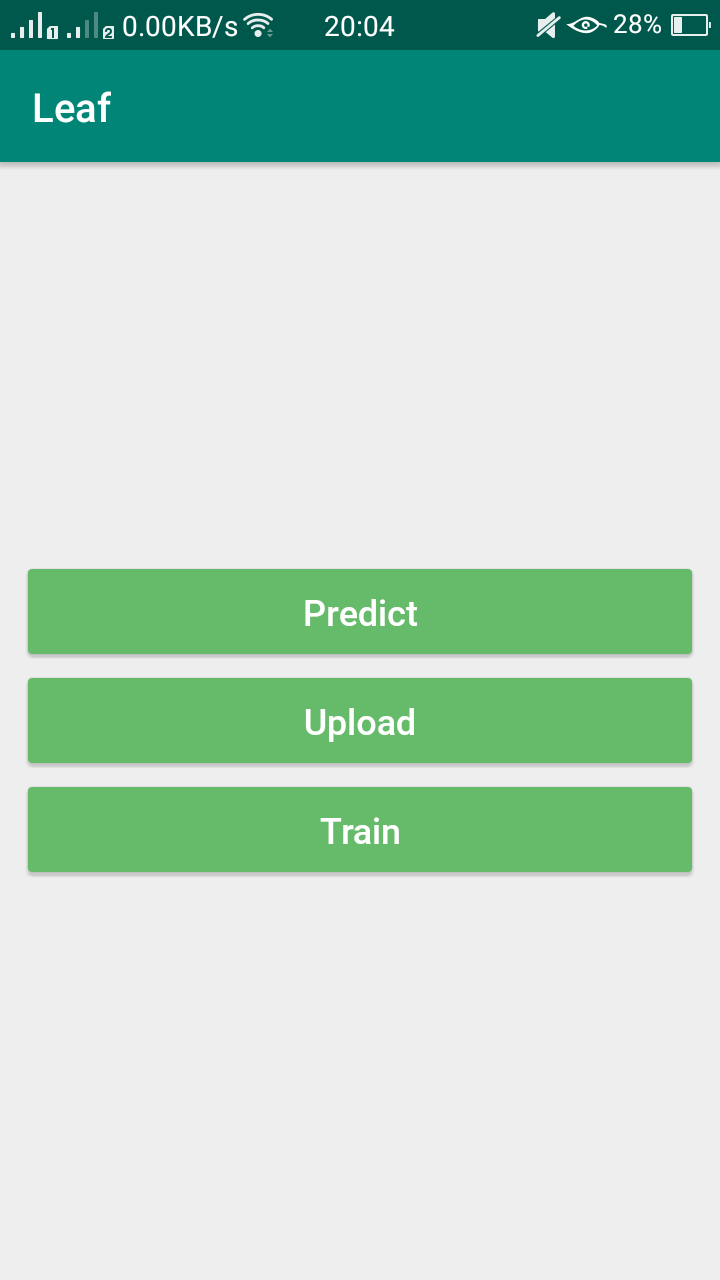
\includegraphics[width=0.5\textwidth]{bab4/figures/main.png}
	\caption{Tampilan awal}
	\label{fig:main}
\end{figure}
\subsection{Implementasi Kelas UploadActivity}
\par Pada kelas UploadActivity pengguna dapat mengunggah gambar beberapa kali dengan nama daun tertentu. Dengan adanya unggahan dari pengguna maka dataset akan bertambah.

\par Fitur Upload menggunakan library \textit{fotoapparat} untuk membuka kamera pada ponsel. Gambar yang ditangkap akan diubah dalam bentuk string sebelum dikirim ke server. Untuk mengirim data ke server digunakan library Retrofit2.

\par Berikut adalah tampilan dari laman upload.
\begin{figure}[H]
	\centering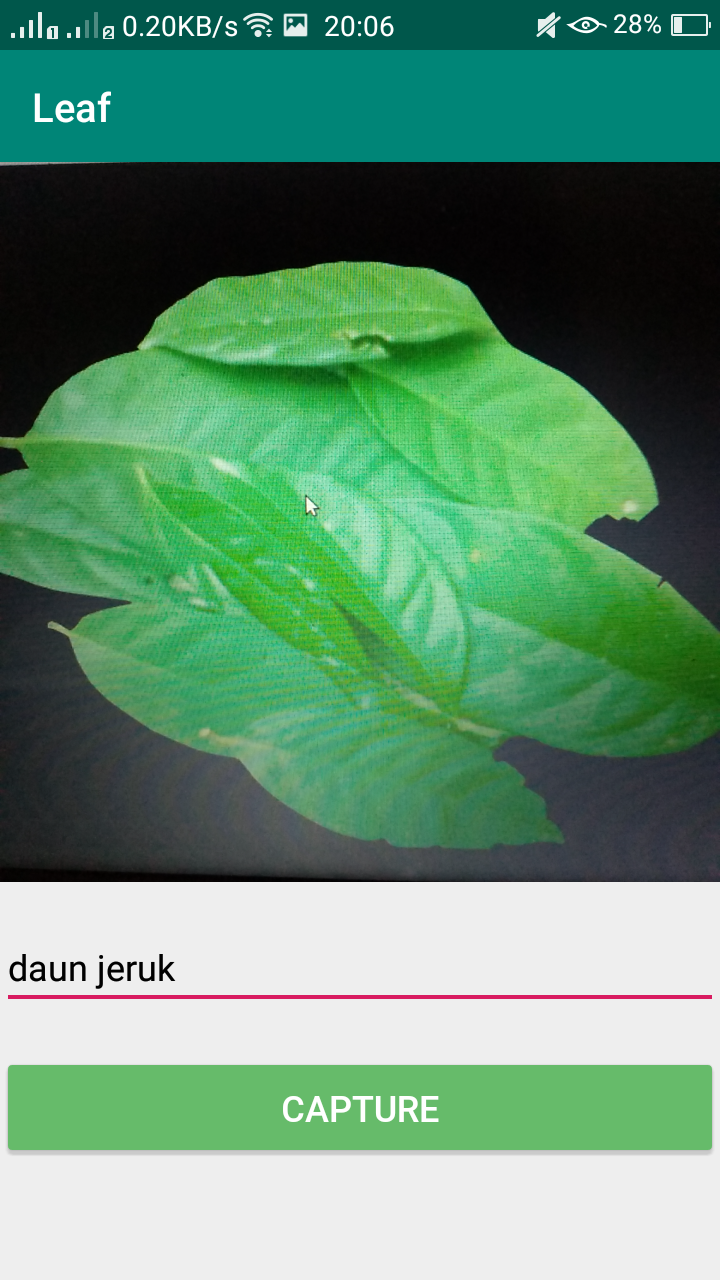
\includegraphics[width=0.5\textwidth]{bab4/figures/upload.png}
	\caption{Tampilan Upload}
	\label{fig:upload}
\end{figure}
\subsection{Implementasi Kelas PredictActivity}

\par Kelas PredictActivity mirip seperti kelas UploadActivity dalam hal tampilan, bedanya adalah kelas ini ketika menembak API pada server akan mendapatkan response berupa nama daun yang diprediksi. Tampilan dari fitur Predict adalah sebagai berikut.
\begin{figure}[H]
	\centering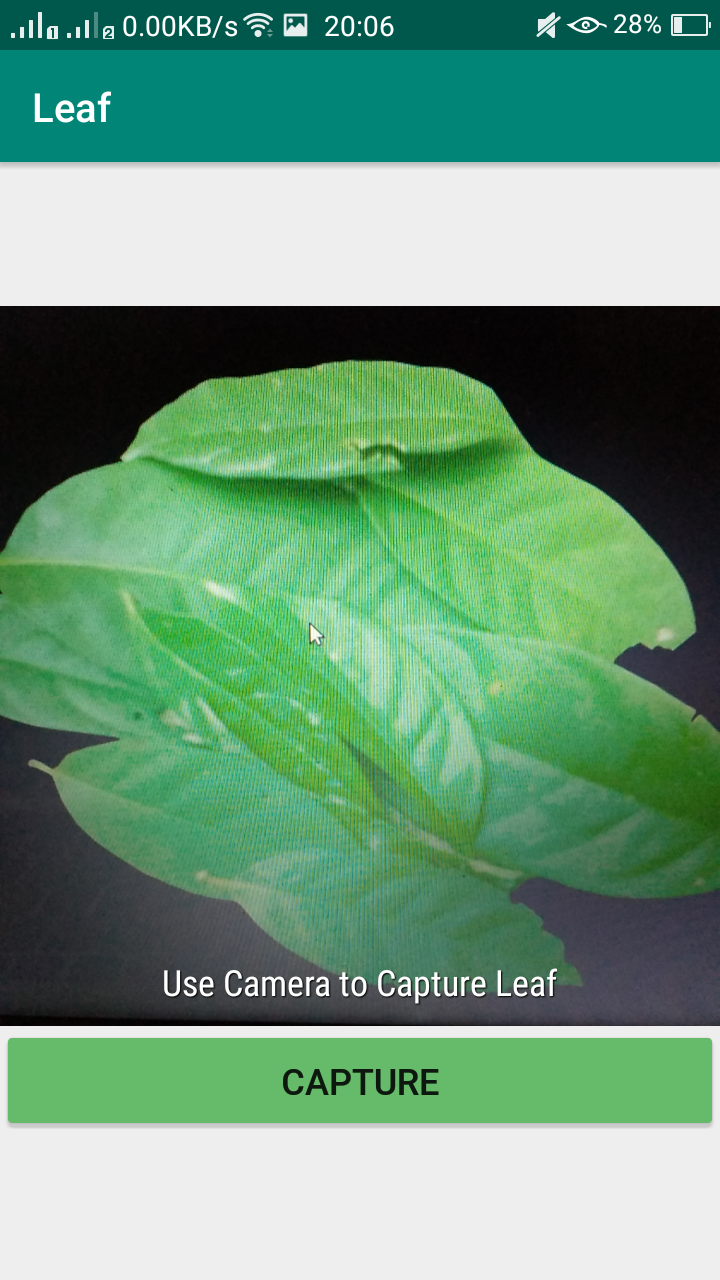
\includegraphics[width=0.5\textwidth]{bab4/figures/predict.png}
	\caption{Tampilan Predict}
	\label{fig:predict}
\end{figure}
\subsection{API}
\par Berikut adalah sumber kode untuk memanggil API pada server.

\begin{lstlisting}[language=python, caption=Pemanggilan API menggunakan Retrofit2, label=code:api, firstnumber=0]
public interface ApiClientAttendance {
@FormUrlEncoded
@POST("/upload/")
Call<ResponseApi> upload(@Field("name") String name,
@Field("image") String image);

@POST("/train/")
Call<ResponseApi> train();

@FormUrlEncoded
@POST("/predict/")
Call<ResponseApi> predict(@Field("image") String image);
}
\end{lstlisting}

\section{Implementasi Backend}
Untuk implementasi backend, yang dibutuhkan adalah \textit{Controller} saja. \textit{Controller} ini yang akan menerima request dan menjalankan program serta mengirim response.
Sumber kode untuk implementasi backend terlampir.